%%%%%%%%%%%%%%%%%%%%%%%%%%%%%%%%%%%%%%%%%
% Beamer Presentation
% LaTeX Template
% Version 1.0 (10/11/12)
%
% This template has been downloaded from:
% http://www.LaTeXTemplates.com
%
% License:
% CC BY-NC-SA 3.0 (http://creativecommons.org/licenses/by-nc-sa/3.0/)
%
%%%%%%%%%%%%%%%%%%%%%%%%%%%%%%%%%%%%%%%%%

%----------------------------------------------------------------------------------------
%	PACKAGES AND THEMES
%----------------------------------------------------------------------------------------

%\documentclass{beamer}
\documentclass[12pt, aspectratio=169]{beamer}
\usepackage{keynote-gradient}

\mode<presentation> {

% The Beamer class comes with a number of default slide themes
% which change the colors and layouts of slides. Below this is a list
% of all the themes, uncomment each in turn to see what they look like.

%\usetheme{default}
%\usetheme{AnnArbor}
%\usetheme{Antibes}
%\usetheme{Bergen}
%\usetheme{Berkeley}
%\usetheme{Berlin}
%\usetheme{Boadilla}
%\usetheme{CambridgeUS}
%\usetheme{Copenhagen}
%\usetheme{Darmstadt}
%\usetheme{Dresden}
%\usetheme{Frankfurt}
%\usetheme{Goettingen}
%\usetheme{Hannover}
%\usetheme{Ilmenau}
%\usetheme{JuanLesPins}
%\usetheme{Luebeck}
%\usetheme{Madrid}
%\usetheme{Malmoe}
%\usetheme{Marburg}
%\usetheme{Montpellier}
%\usetheme{PaloAlto}
%\usetheme{Pittsburgh}
%\usetheme{Rochester}
%\usetheme{Singapore}
%\usetheme{Szeged}
%\usetheme{Warsaw}

% As well as themes, the Beamer class has a number of color themes
% for any slide theme. Uncomment each of these in turn to see how it
% changes the colors of your current slide theme.

%\usecolortheme{albatross}
%\usecolortheme{beaver}
%\usecolortheme{beetle}
%\usecolortheme{crane}
%\usecolortheme{dolphin}
%\usecolortheme{dove}
%\usecolortheme{fly}
%\usecolortheme{lily}
%\usecolortheme{orchid}
%\usecolortheme{rose}
%\usecolortheme{seagull}
%\usecolortheme{seahorse}
%\usecolortheme{whale}
%\usecolortheme{wolverine}

%\setbeamertemplate{footline} % To remove the footer line in all slides uncomment this line
\setbeamertemplate{footline}[page number] % To replace the footer line in all slides with a simple slide count uncomment this line

\setbeamertemplate{navigation symbols}{} % To remove the navigation symbols from the bottom of all slides uncomment this line
}

\usepackage{graphicx} % Allows including images
\usepackage{booktabs} % Allows the use of \toprule, \midrule and \bottomrule in tables

%----------------------------------------------------------------------------------------
%	TITLE PAGE
%----------------------------------------------------------------------------------------

\title[MCL projects]{Machine Cognition Lab projects: \\Neuromorphic Robot Dream} % The short title appears at the bottom of every slide, the full title is only on the title page

\author[Max Talanov]{
  
\includegraphics[height=3cm]{ITIS_logo_bright}\\
  Max Talanov
} 
\institute[ITIS: KFU] % Your institution as it will appear on the bottom of every slide, may be shorthand to save space
{
Machine cognition lab, Intellectual robotics department, ITIS \\ % Your institution for the title page
\medskip
\textit{max.talanov@gmail.com} % Your email address
}
\date{\today} % Date, can be changed to a custom date

\begin{document}

\begin{frame}
\titlepage % Print the title page as the first slide
\end{frame}


%----------------------------------------------------------------------------------------
%	PRESENTATION SLIDES
%----------------------------------------------------------------------------------------

%------------------------------------------------
\section{The consciousness} % Sections can be created in order to organize your presentation into discrete blocks, all sections and subsections are automatically printed in the table of contents as an overview of the talk
%------------------------------------------------
%------------------------------------------------

\begin{frame}
\frametitle{Consciousness $\Rightarrow$ Emotions}
\begin{columns}[c] % The "c" option specifies centered vertical alignment while the "t" option is used for top vertical alignment

\column{.45\textwidth} % Left column and width
\textbf{Human:}
\begin{itemize}
\item Cognition $\Rightarrow$ Consciousness $\Rightarrow$ Emotions
\end{itemize}

\textbf{Machine:}
\begin{itemize}
\item Cognition $\Rightarrow$ Consciousness $\Rightarrow$ Emotions
\end{itemize}

\column{.6\textwidth} % Right column and width
%------------------------------------------------
\begin{figure}
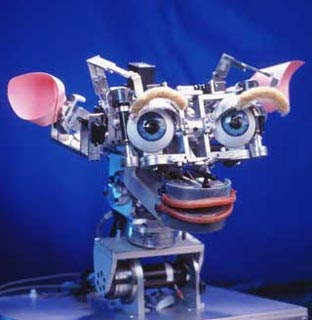
\includegraphics[width=0.8\linewidth]{Kismet_312}
\end{figure}
%------------------------------------------------
\end{columns}
\end{frame}

%------------------------------------------------

\begin{frame}
\frametitle{Robot emotions}
\begin{figure}
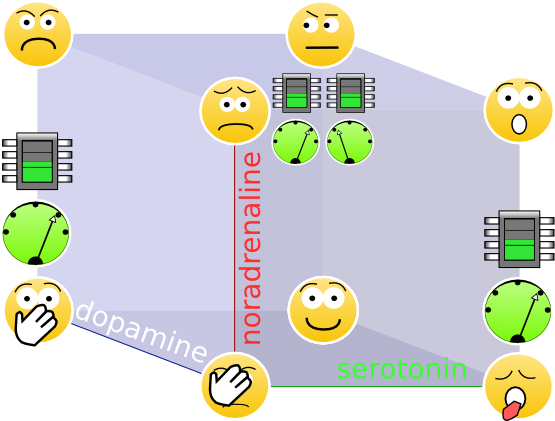
\includegraphics[width=0.7\linewidth]{cube_of_emotional_parameters_machine}
\end{figure}
%------------------------------------------------
\end{frame}

%------------------------------------------------

\begin{frame}
\frametitle{Experiment}
\begin{figure}
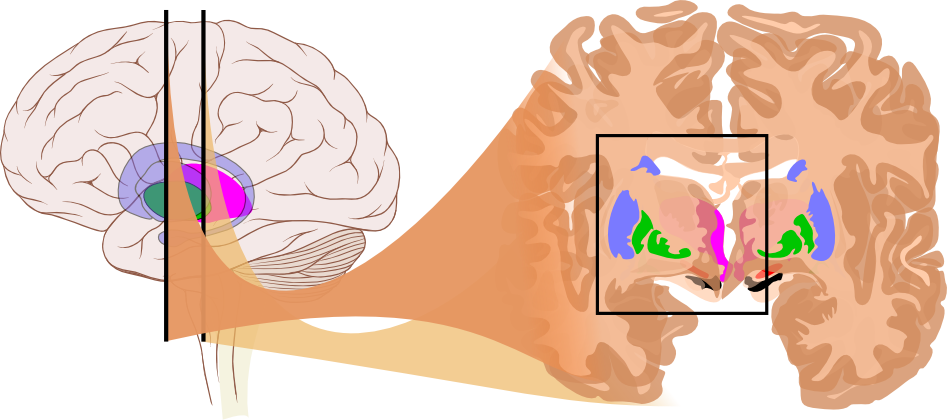
\includegraphics[width=0.99\linewidth]{Basal_ganglia_circuits_cropped}
\end{figure}
\end{frame}

%------------------------------------------------

\begin{frame}
\frametitle{Dopamine pathways diagram}
\begin{figure}
\includegraphics[width=0.8\linewidth]{dopamine_diagram}
\end{figure}
\end{frame}

%------------------------------------------------


\begin{frame}
\frametitle{Results}
\begin{figure}
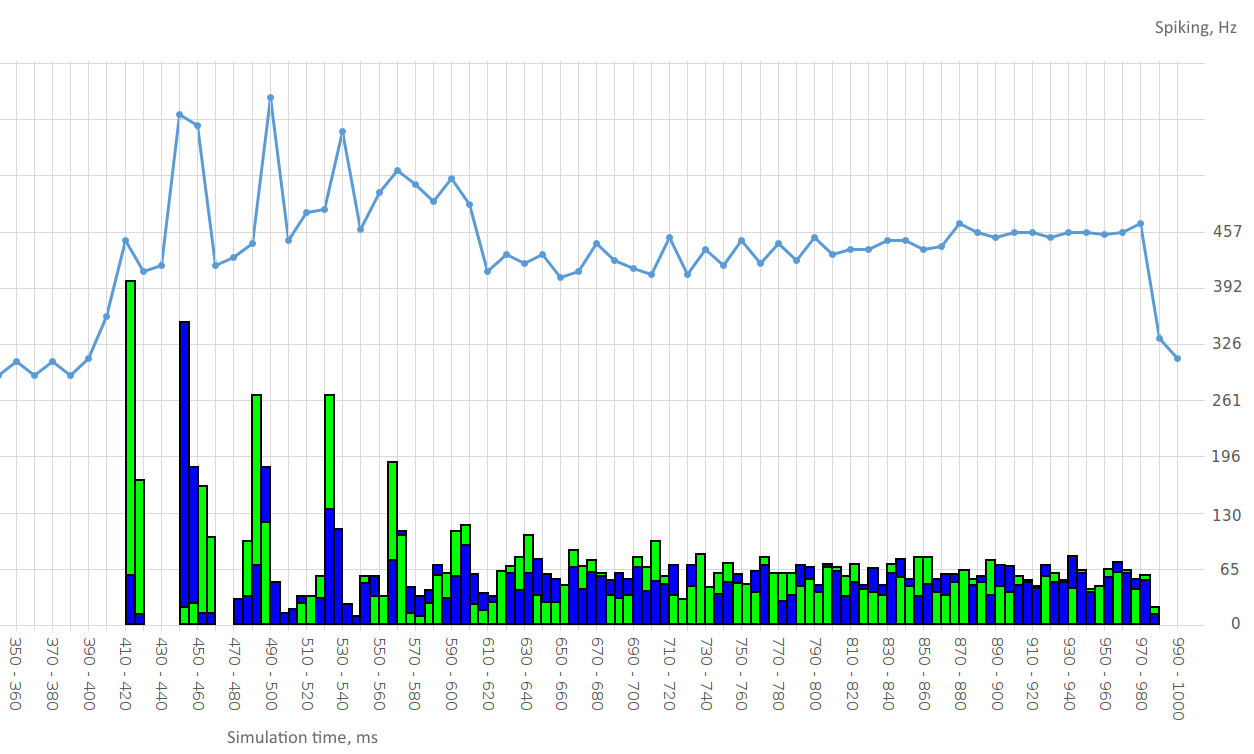
\includegraphics[width=0.8\linewidth]{resultBIG_short}
\end{figure}
\end{frame}


%------------------------------------------------

\begin{frame}
\frametitle{Robot performance}
\begin{columns}[c] % The "c" option specifies centered vertical alignment while the "t" option is used for top vertical alignment

\column{.45\textwidth} % Left column and width
\begin{itemize}
\item \textbf{AR-601}: Intel Core i7-4700EQ; 8 GB;
\item \textbf{REEM-C}: Intel Core i7 2710QE x 2;
\item \textbf{Nao}: Intel Atom @ 1.6 GHz;
\item \textbf{iCub}: Intel® Core™2 Duo; 2 GB;
\end{itemize}


\column{.6\textwidth} % Right column and width
%------------------------------------------------
\begin{figure}
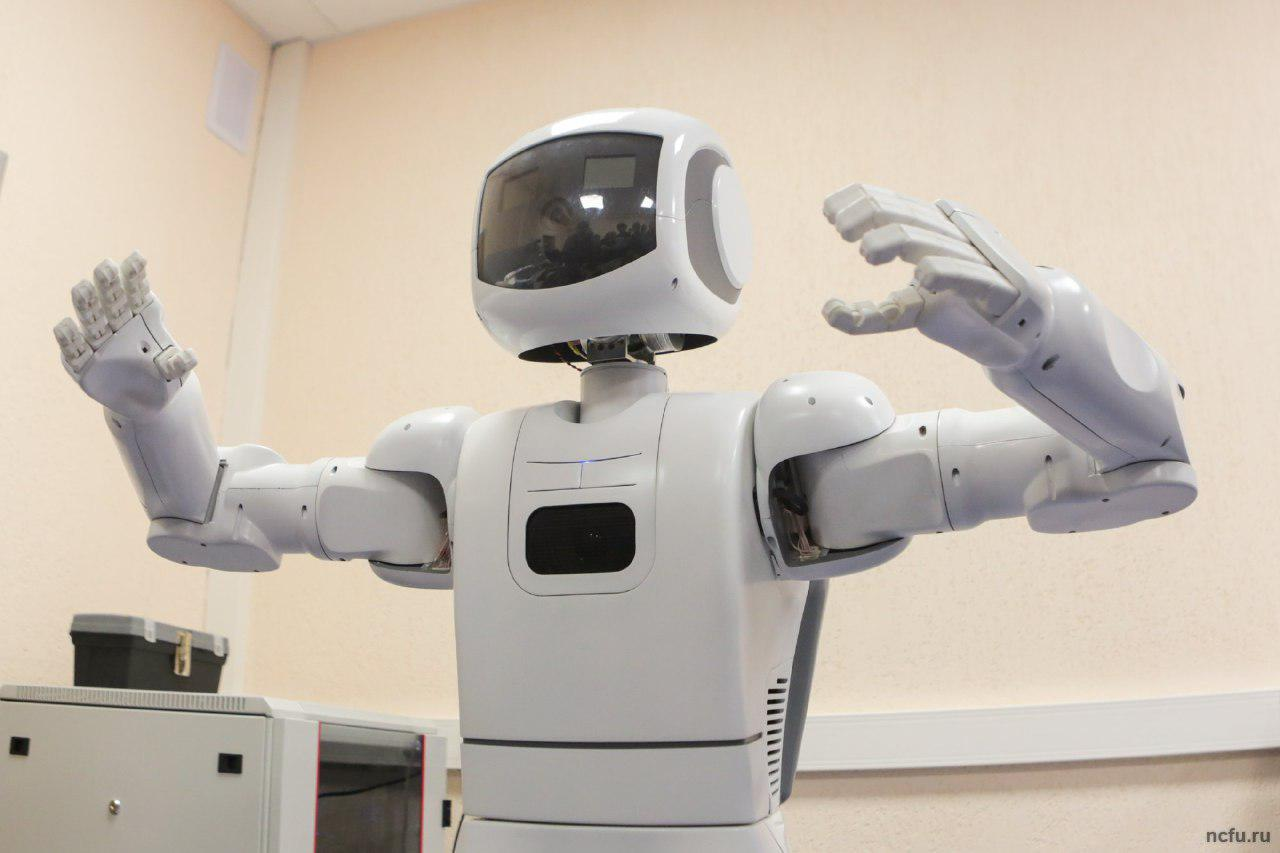
\includegraphics[width=1.0\linewidth]{AR-601}
\end{figure}
%------------------------------------------------
\end{columns}
\end{frame}

%------------------------------------------------

\begin{frame}
\frametitle{Performance that we need}
\begin{columns}[c] % The "c" option specifies centered vertical alignment while the "t" option is used for top vertical alignment

\column{.45\textwidth} % Left column and width
\textbf{RIKEN} 2013: 1\% of human brain - 250 K-supercomputers
(96 computing nodes, 2.0 GHz 8-core SPARC64; 16 GB of memory), slower than human brain in 1000 times. 

\textbf{Human brain project}: a whole human brain -- 10 exaflop.


\column{.6\textwidth} % Right column and width
%------------------------------------------------
\begin{figure}
\includegraphics[width=1.0\linewidth]{RIKEN_AICS}
\end{figure}
%------------------------------------------------
\end{columns}
\end{frame}


%------------------------------------------------
\section{Solution}
%------------------------------------------------

\begin{frame}
\frametitle{Robot dream}
\begin{figure}
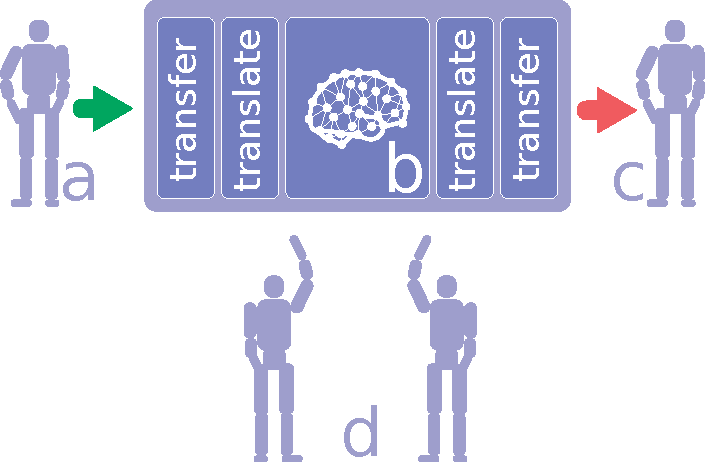
\includegraphics[width=0.8\linewidth]{robot-dream}
\end{figure}
\end{frame}

%------------------------------------------------

\begin{frame}
\frametitle{Preliminary results}
\begin{figure}
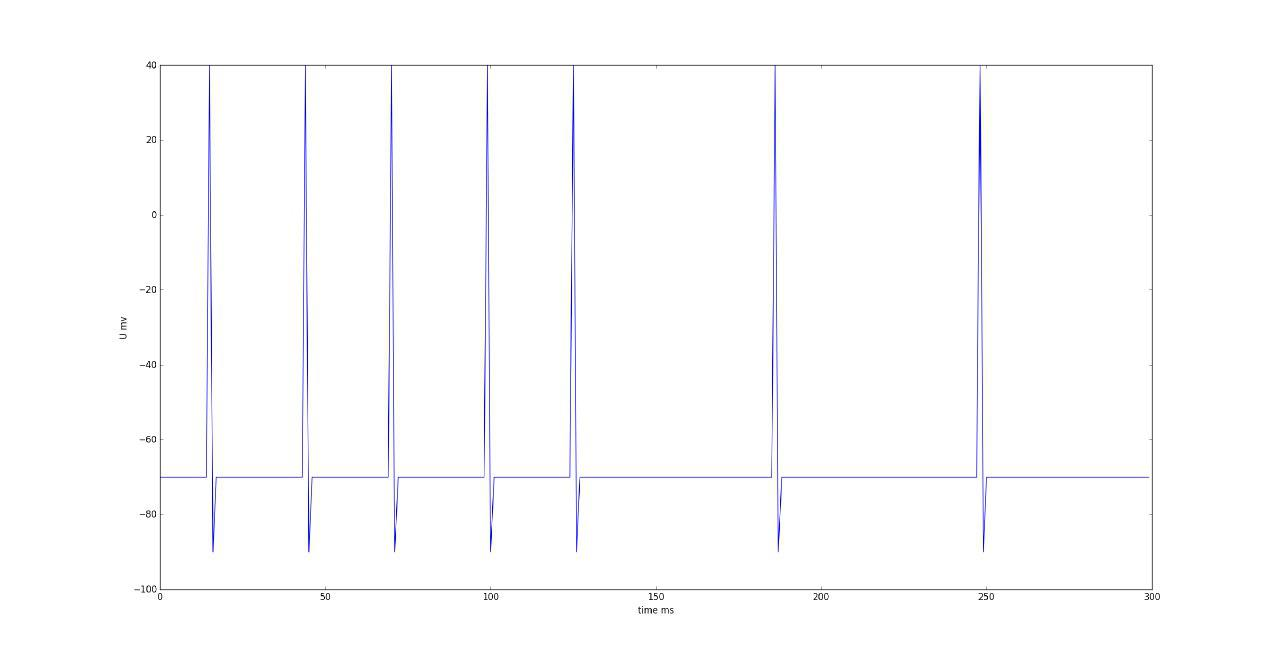
\includegraphics[width=0.8\linewidth]{pseudo-neuronal-activity}
\end{figure}
\end{frame}

%------------------------------------------------

%------------------------------------------------

\begin{frame}
\frametitle{Memristive solution for "wake" system}
\begin{figure}
\includegraphics[width=0.8\linewidth]{HL_Emristor}
\end{figure}
\end{frame}

%------------------------------------------------



\begin{frame}
  \frametitle{Future work}
  
\begin{itemize}
  \item Simple prototype as feasibility study.
  \item \ldots\
  \item Emotional robot with real-time embodiment
  \item Social robot with emotions
  \item Conscious social robot
\end{itemize}

\textbf{Acknowledgment}

Part of the work was performed according to the Russian Government Program of Competitive Growth of Kazan Federal University.

\end{frame}

%------------------------------------------------


%------------------------------------------------

\end{document} 
